\documentclass[]{article}
\usepackage{lmodern}
\usepackage{amssymb,amsmath}
\usepackage{ifxetex,ifluatex}
\usepackage{fixltx2e} % provides \textsubscript
\ifnum 0\ifxetex 1\fi\ifluatex 1\fi=0 % if pdftex
  \usepackage[T1]{fontenc}
  \usepackage[utf8]{inputenc}
\else % if luatex or xelatex
  \ifxetex
    \usepackage{mathspec}
  \else
    \usepackage{fontspec}
  \fi
  \defaultfontfeatures{Ligatures=TeX,Scale=MatchLowercase}
\fi
% use upquote if available, for straight quotes in verbatim environments
\IfFileExists{upquote.sty}{\usepackage{upquote}}{}
% use microtype if available
\IfFileExists{microtype.sty}{%
\usepackage{microtype}
\UseMicrotypeSet[protrusion]{basicmath} % disable protrusion for tt fonts
}{}
\usepackage[margin=1in]{geometry}
\usepackage{hyperref}
\PassOptionsToPackage{usenames,dvipsnames}{color} % color is loaded by hyperref
\hypersetup{unicode=true,
            pdftitle={K-means Clustering},
            colorlinks=true,
            linkcolor=Maroon,
            citecolor=Blue,
            urlcolor=blue,
            breaklinks=true}
\urlstyle{same}  % don't use monospace font for urls
\usepackage{color}
\usepackage{fancyvrb}
\newcommand{\VerbBar}{|}
\newcommand{\VERB}{\Verb[commandchars=\\\{\}]}
\DefineVerbatimEnvironment{Highlighting}{Verbatim}{commandchars=\\\{\}}
% Add ',fontsize=\small' for more characters per line
\usepackage{framed}
\definecolor{shadecolor}{RGB}{248,248,248}
\newenvironment{Shaded}{\begin{snugshade}}{\end{snugshade}}
\newcommand{\KeywordTok}[1]{\textcolor[rgb]{0.13,0.29,0.53}{\textbf{#1}}}
\newcommand{\DataTypeTok}[1]{\textcolor[rgb]{0.13,0.29,0.53}{#1}}
\newcommand{\DecValTok}[1]{\textcolor[rgb]{0.00,0.00,0.81}{#1}}
\newcommand{\BaseNTok}[1]{\textcolor[rgb]{0.00,0.00,0.81}{#1}}
\newcommand{\FloatTok}[1]{\textcolor[rgb]{0.00,0.00,0.81}{#1}}
\newcommand{\ConstantTok}[1]{\textcolor[rgb]{0.00,0.00,0.00}{#1}}
\newcommand{\CharTok}[1]{\textcolor[rgb]{0.31,0.60,0.02}{#1}}
\newcommand{\SpecialCharTok}[1]{\textcolor[rgb]{0.00,0.00,0.00}{#1}}
\newcommand{\StringTok}[1]{\textcolor[rgb]{0.31,0.60,0.02}{#1}}
\newcommand{\VerbatimStringTok}[1]{\textcolor[rgb]{0.31,0.60,0.02}{#1}}
\newcommand{\SpecialStringTok}[1]{\textcolor[rgb]{0.31,0.60,0.02}{#1}}
\newcommand{\ImportTok}[1]{#1}
\newcommand{\CommentTok}[1]{\textcolor[rgb]{0.56,0.35,0.01}{\textit{#1}}}
\newcommand{\DocumentationTok}[1]{\textcolor[rgb]{0.56,0.35,0.01}{\textbf{\textit{#1}}}}
\newcommand{\AnnotationTok}[1]{\textcolor[rgb]{0.56,0.35,0.01}{\textbf{\textit{#1}}}}
\newcommand{\CommentVarTok}[1]{\textcolor[rgb]{0.56,0.35,0.01}{\textbf{\textit{#1}}}}
\newcommand{\OtherTok}[1]{\textcolor[rgb]{0.56,0.35,0.01}{#1}}
\newcommand{\FunctionTok}[1]{\textcolor[rgb]{0.00,0.00,0.00}{#1}}
\newcommand{\VariableTok}[1]{\textcolor[rgb]{0.00,0.00,0.00}{#1}}
\newcommand{\ControlFlowTok}[1]{\textcolor[rgb]{0.13,0.29,0.53}{\textbf{#1}}}
\newcommand{\OperatorTok}[1]{\textcolor[rgb]{0.81,0.36,0.00}{\textbf{#1}}}
\newcommand{\BuiltInTok}[1]{#1}
\newcommand{\ExtensionTok}[1]{#1}
\newcommand{\PreprocessorTok}[1]{\textcolor[rgb]{0.56,0.35,0.01}{\textit{#1}}}
\newcommand{\AttributeTok}[1]{\textcolor[rgb]{0.77,0.63,0.00}{#1}}
\newcommand{\RegionMarkerTok}[1]{#1}
\newcommand{\InformationTok}[1]{\textcolor[rgb]{0.56,0.35,0.01}{\textbf{\textit{#1}}}}
\newcommand{\WarningTok}[1]{\textcolor[rgb]{0.56,0.35,0.01}{\textbf{\textit{#1}}}}
\newcommand{\AlertTok}[1]{\textcolor[rgb]{0.94,0.16,0.16}{#1}}
\newcommand{\ErrorTok}[1]{\textcolor[rgb]{0.64,0.00,0.00}{\textbf{#1}}}
\newcommand{\NormalTok}[1]{#1}
\usepackage{graphicx,grffile}
\makeatletter
\def\maxwidth{\ifdim\Gin@nat@width>\linewidth\linewidth\else\Gin@nat@width\fi}
\def\maxheight{\ifdim\Gin@nat@height>\textheight\textheight\else\Gin@nat@height\fi}
\makeatother
% Scale images if necessary, so that they will not overflow the page
% margins by default, and it is still possible to overwrite the defaults
% using explicit options in \includegraphics[width, height, ...]{}
\setkeys{Gin}{width=\maxwidth,height=\maxheight,keepaspectratio}
\IfFileExists{parskip.sty}{%
\usepackage{parskip}
}{% else
\setlength{\parindent}{0pt}
\setlength{\parskip}{6pt plus 2pt minus 1pt}
}
\setlength{\emergencystretch}{3em}  % prevent overfull lines
\providecommand{\tightlist}{%
  \setlength{\itemsep}{0pt}\setlength{\parskip}{0pt}}
\setcounter{secnumdepth}{5}
% Redefines (sub)paragraphs to behave more like sections
\ifx\paragraph\undefined\else
\let\oldparagraph\paragraph
\renewcommand{\paragraph}[1]{\oldparagraph{#1}\mbox{}}
\fi
\ifx\subparagraph\undefined\else
\let\oldsubparagraph\subparagraph
\renewcommand{\subparagraph}[1]{\oldsubparagraph{#1}\mbox{}}
\fi

%%% Use protect on footnotes to avoid problems with footnotes in titles
\let\rmarkdownfootnote\footnote%
\def\footnote{\protect\rmarkdownfootnote}

%%% Change title format to be more compact
\usepackage{titling}

% Create subtitle command for use in maketitle
\providecommand{\subtitle}[1]{
  \posttitle{
    \begin{center}\large#1\end{center}
    }
}

\setlength{\droptitle}{-2em}

  \title{K-means Clustering}
    \pretitle{\vspace{\droptitle}\centering\huge}
  \posttitle{\par}
    \author{}
    \preauthor{}\postauthor{}
    \date{}
    \predate{}\postdate{}
  
\usepackage{graphicx}
\usepackage{float}

\begin{document}
\maketitle

\section{Short Intro}\label{short-intro}

K-means clustering is an unsupervised machine learning algorithm.
Unsupervised algorithms make inferences using only input data without
referring to known, or labeled outcomes. The goal of the K-means is to
group similar observations together and discover underlying patterns.

An input to the K-means algorithm is a number \textbf{k}, which refers
to the number of groups (clusters) that the observations will be grouped
into. The algorithm actually finds centers of those clusters (called
\emph{centroids}) and allocates each observation to the nearest cluster.
The objective of the K-means is to minimize the in-cluster sum of
squares, that is the sum of the squared distance of every point to its
corresponding cluster centroid.

Steps of the K-means algorithm:

\begin{enumerate}
\def\labelenumi{\arabic{enumi})}
\tightlist
\item
  The initial selection of cluster centroids. Centroids are either
  randomly generated or selected from the data set, i.e.~K random
  observations are declared as centroids
\end{enumerate}

Repeat:

\begin{enumerate}
\def\labelenumi{\arabic{enumi})}
\setcounter{enumi}{1}
\item
  Cluster assignment: For each instance from the data set, identify the
  nearest centroid (usually based on the Euclidean distance) and assign
  the instance to the cluster of that centroid.
\item
  Centroid update: for each cluster, calculate a new centroid by taking
  the mean of all data points assigned to that centroid's cluster.
\end{enumerate}

The algorithm iterates between steps 2 and 3 until no data points change
clusters, the sum of the distances is minimized, or a maximum number of
iterations is reached.

The result may be a local optimum (which may not necessarily be the best
possible outcome). This means that running the algorithm with randomized
starting centroids may give better results.

\subsection{K-means Example}\label{k-means-example}

Suppose we have a dataset with several observations and two variables.
They can be plotted in the Euclidean space (Fig. 1).

\begin{figure}[H]

{\centering 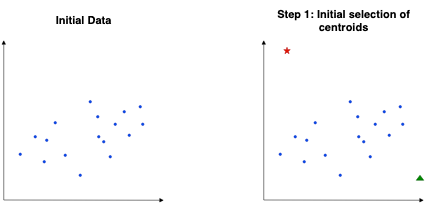
\includegraphics[width=350px]{images/steps_0_1} 

}

\caption{Initial data and Initial selection of centroids}\label{fig:unnamed-chunk-2}
\end{figure}

In the \textbf{Step 1} of the algorithm, we randomly choose the
centroids. Suppose k=2, which means we need to choose two centroids.
Although there are other approaches to choosing centroids, we will use
the most basic one: choosing randomly. Still, it is advisable to
generate the most disperse values possible (maximizing distance between
centroids) in order to prevent unwanted localized convergence.

In the \textbf{Step 2}, we assign a cluster to each observation (Fig.
2). The assignment is performed based on the Euclidean distance measured
from a data point (representing the observation) to centroids. An
observation is assigned the cluster of the nearest centroid.

In the \textbf{Step 3}, we update the cluster centroids and assign them
a new value based on the mean value of all observations that belong to
the cluster (Fig. 2).

\begin{figure}[H]

{\centering 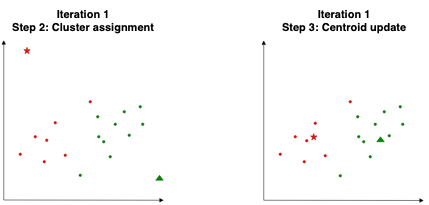
\includegraphics[width=350px]{images/steps_2_3_iter1} 

}

\caption{Cluster assignment and centroid update (Iteration 1)}\label{fig:unnamed-chunk-3}
\end{figure}

In the next iteration (Iteration 2), we repeat Steps 2 and 3 (Fig. 3).
In the \textbf{Step 2}, we again assign each data point (observation)
with a cluster. We can observe that two data points changed their
cluster, i.e.~they switched the cluster. After that, in the \textbf{Step
3}, we again calculate new centroid positions with the mean value of all
the observations that currently belong to the corresponding clusters.

\begin{figure}[H]

{\centering 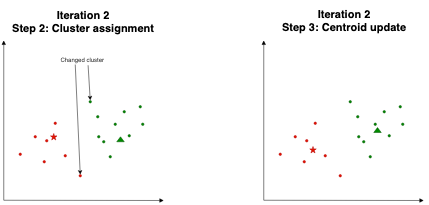
\includegraphics[width=350px]{images/steps_2_3_iter2} 

}

\caption{Cluster assignment and centroid update (Iteration 2)}\label{fig:unnamed-chunk-4}
\end{figure}

In Iteration 3, none of the observations would change their cluster.
This means that the algorithm has converged and that no further
iterations should be performed.

\section{Load and prepare data set}\label{load-and-prepare-data-set}

\emph{Wholesale Customer dataset} contains data about clients of a
wholesale distributor. It includes the annual spending in monetary units
(m.u.) on diverse product categories. The dataset is available from the
\href{https://archive.ics.uci.edu/ml/datasets/Wholesale+customers}{UCI
ML Repository} (the dataset used in this script is partially
preprocessed, where \emph{Channel} and \emph{Region} attributes are
factorized and outliers were removed for some variables).

The objective is to segment (cluster) customers.

Let's load the dataset.

\begin{Shaded}
\begin{Highlighting}[]
\CommentTok{# load the data from "data/wholesale_customers.csv"}
\NormalTok{customers.data <-}\StringTok{ }\KeywordTok{read.csv}\NormalTok{(}\DataTypeTok{file =} \StringTok{"data/wholesale_customers.csv"}\NormalTok{)}

\CommentTok{# print the structure}
\KeywordTok{str}\NormalTok{(customers.data)}
\end{Highlighting}
\end{Shaded}

\begin{verbatim}
## 'data.frame':    440 obs. of  8 variables:
##  $ Channel         : Factor w/ 2 levels "Horeca","Retail": 2 2 2 1 2 2 2 2 1 2 ...
##  $ Region          : Factor w/ 3 levels "Lisbon","Oporto",..: 3 3 3 3 3 3 3 3 3 3 ...
##  $ Fresh           : num  12669 7057 6353 13265 22615 ...
##  $ Milk            : num  9656 9810 8808 1196 5410 ...
##  $ Grocery         : int  7561 9568 7684 4221 7198 5126 6975 9426 6192 18881 ...
##  $ Frozen          : num  214 1762 2405 6404 3915 ...
##  $ Detergents_Paper: num  2674 3293 3516 507 1777 ...
##  $ Delicatessen    : num  1338 1776 3456 1788 3456 ...
\end{verbatim}

\subsection{Examining and Preparing the
Data}\label{examining-and-preparing-the-data}

We will first check if there are observations with missing values. If
missing values are present, those instances should be either removed or
imputed (imputation is the process of replacing missing data with
substituted values).

\begin{Shaded}
\begin{Highlighting}[]
\CommentTok{# check for missing values}
\KeywordTok{which}\NormalTok{(}\KeywordTok{complete.cases}\NormalTok{(customers.data)}\OperatorTok{==}\NormalTok{F)}
\end{Highlighting}
\end{Shaded}

\begin{verbatim}
## integer(0)
\end{verbatim}

In our dataset, there are no missing values.

Since the algorithm is based on measuring distances (e.g.~Euclidean),
this implies that \textbf{all variables must be continuous} and the
approach can be severely \textbf{affected by outliers}. So, we should
check if outliers are present. We will check only numerical variables
that will be used for clustering.

Box-plots are useful for the detection of outliers. More details on how
to analyze the box plot can be found
\href{https://flowingdata.com/2008/02/15/how-to-read-and-use-a-box-and-whisker-plot/}{here}.

\begin{Shaded}
\begin{Highlighting}[]
\CommentTok{# plot boxplots for all numeric variables}
\KeywordTok{ggplot}\NormalTok{(customers.data, }\KeywordTok{aes}\NormalTok{(}\DataTypeTok{x=}\NormalTok{Channel, }\DataTypeTok{y=}\NormalTok{Grocery, }\DataTypeTok{fill=}\NormalTok{Channel)) }\OperatorTok{+}\StringTok{ }\KeywordTok{geom_boxplot}\NormalTok{()}
\end{Highlighting}
\end{Shaded}

\begin{center}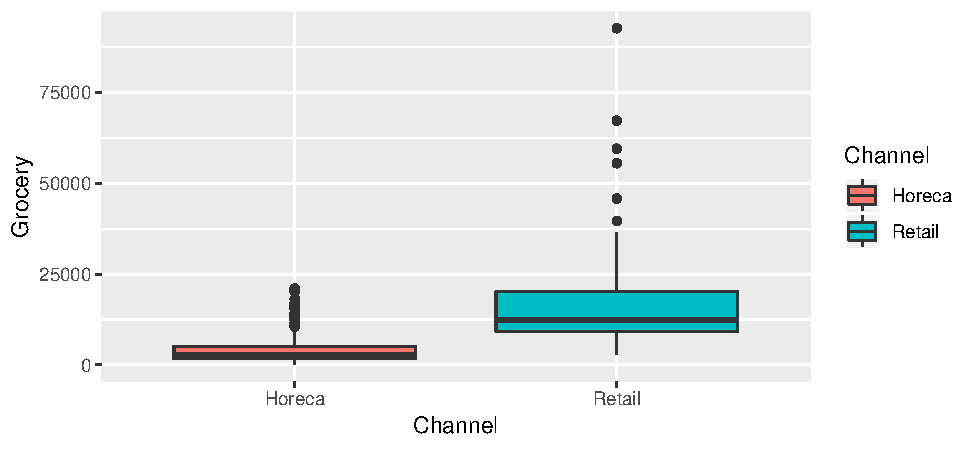
\includegraphics{7._K-means_Clustering_files/figure-latex/unnamed-chunk-8-1} \end{center}

\begin{Shaded}
\begin{Highlighting}[]
\KeywordTok{ggplot}\NormalTok{(customers.data, }\KeywordTok{aes}\NormalTok{(}\DataTypeTok{x=}\NormalTok{Channel, }\DataTypeTok{y=}\NormalTok{Milk, }\DataTypeTok{fill=}\NormalTok{Channel)) }\OperatorTok{+}\StringTok{ }\KeywordTok{geom_boxplot}\NormalTok{()}
\end{Highlighting}
\end{Shaded}

\begin{center}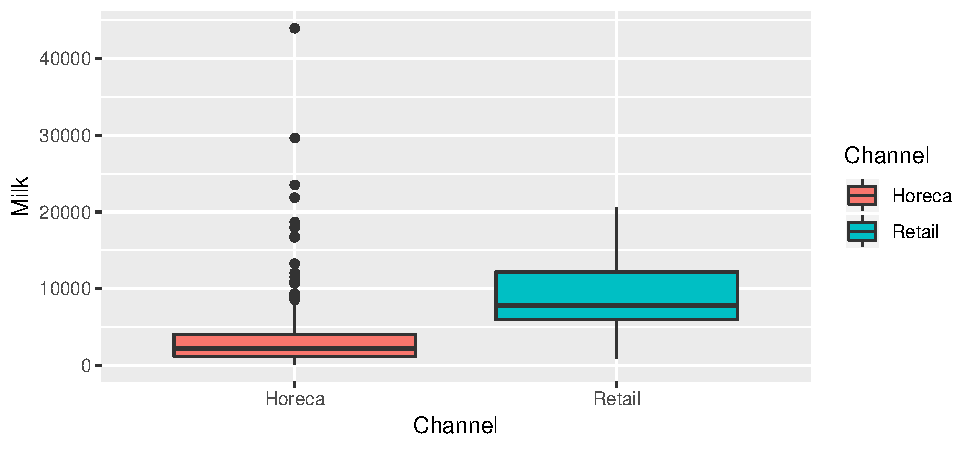
\includegraphics{7._K-means_Clustering_files/figure-latex/unnamed-chunk-8-2} \end{center}

\begin{Shaded}
\begin{Highlighting}[]
\KeywordTok{ggplot}\NormalTok{(customers.data, }\KeywordTok{aes}\NormalTok{(}\DataTypeTok{x=}\NormalTok{Channel, }\DataTypeTok{y=}\NormalTok{Delicatessen, }\DataTypeTok{fill=}\NormalTok{Channel)) }\OperatorTok{+}\StringTok{ }\KeywordTok{geom_boxplot}\NormalTok{()}
\end{Highlighting}
\end{Shaded}

\begin{center}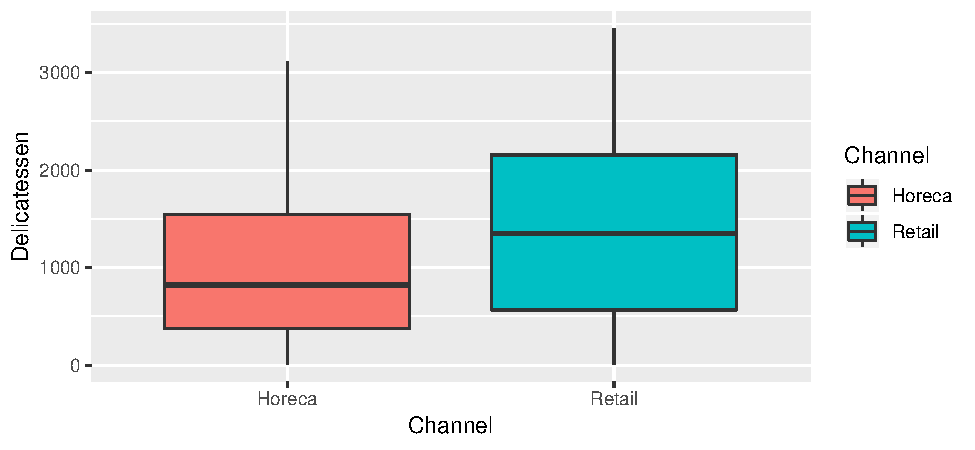
\includegraphics{7._K-means_Clustering_files/figure-latex/unnamed-chunk-8-3} \end{center}

\begin{Shaded}
\begin{Highlighting}[]
\KeywordTok{ggplot}\NormalTok{(customers.data, }\KeywordTok{aes}\NormalTok{(}\DataTypeTok{x=}\NormalTok{Channel, }\DataTypeTok{y=}\NormalTok{Frozen, }\DataTypeTok{fill=}\NormalTok{Channel)) }\OperatorTok{+}\StringTok{ }\KeywordTok{geom_boxplot}\NormalTok{()}
\end{Highlighting}
\end{Shaded}

\begin{center}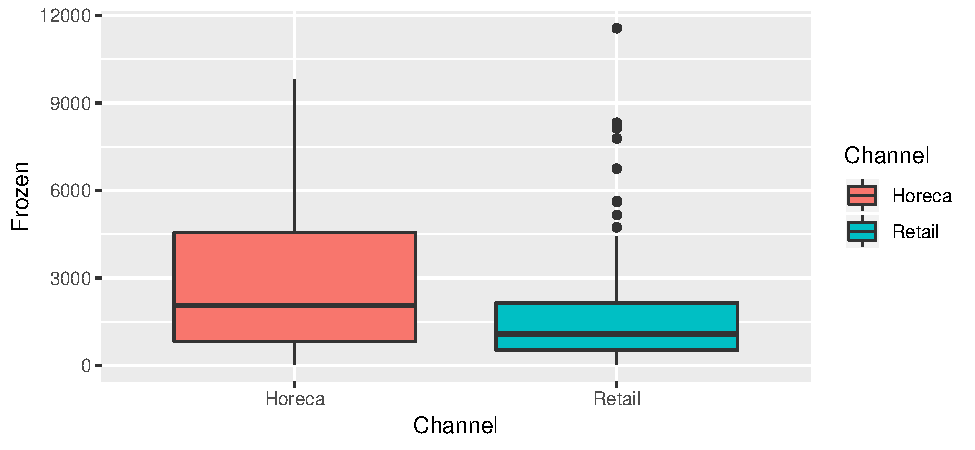
\includegraphics{7._K-means_Clustering_files/figure-latex/unnamed-chunk-8-4} \end{center}

\begin{Shaded}
\begin{Highlighting}[]
\KeywordTok{ggplot}\NormalTok{(customers.data, }\KeywordTok{aes}\NormalTok{(}\DataTypeTok{x=}\NormalTok{Channel, }\DataTypeTok{y=}\NormalTok{Fresh, }\DataTypeTok{fill=}\NormalTok{Channel)) }\OperatorTok{+}\StringTok{ }\KeywordTok{geom_boxplot}\NormalTok{()}
\end{Highlighting}
\end{Shaded}

\begin{center}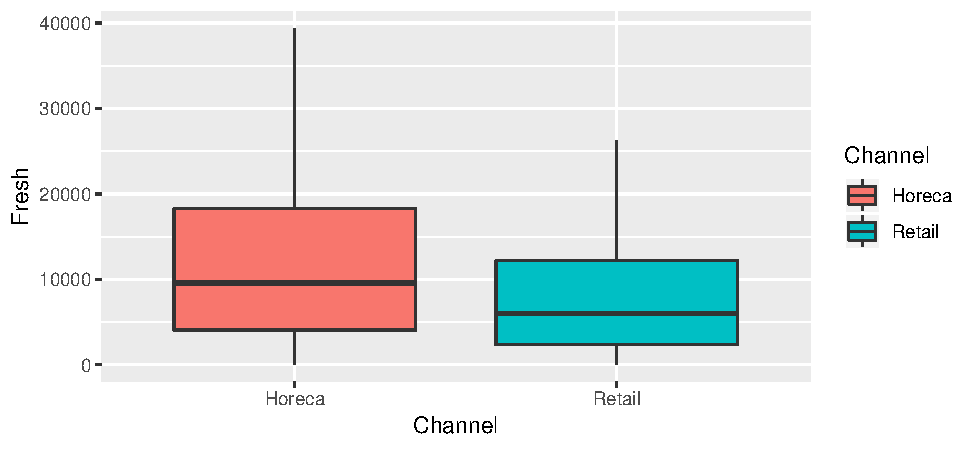
\includegraphics{7._K-means_Clustering_files/figure-latex/unnamed-chunk-8-5} \end{center}

\begin{Shaded}
\begin{Highlighting}[]
\KeywordTok{ggplot}\NormalTok{(customers.data, }\KeywordTok{aes}\NormalTok{(}\DataTypeTok{x=}\NormalTok{Channel, }\DataTypeTok{y=}\NormalTok{Detergents_Paper, }\DataTypeTok{fill=}\NormalTok{Channel)) }\OperatorTok{+}\StringTok{ }\KeywordTok{geom_boxplot}\NormalTok{()}
\end{Highlighting}
\end{Shaded}

\begin{center}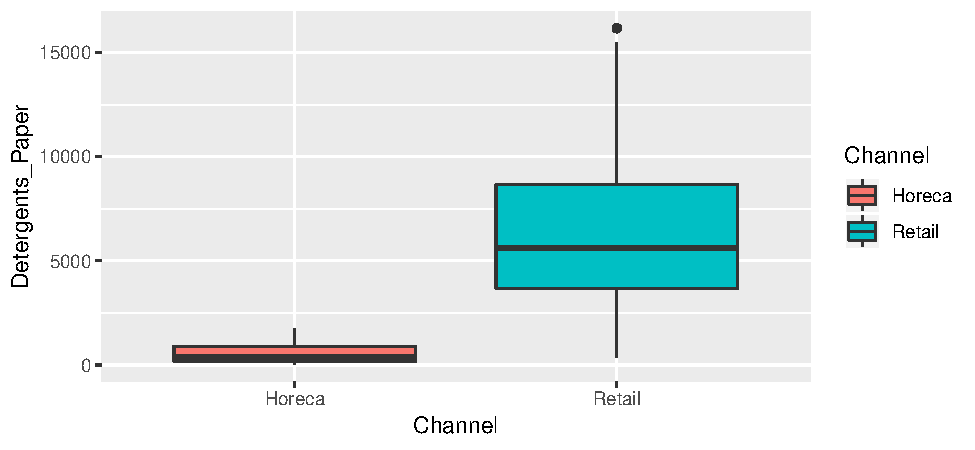
\includegraphics{7._K-means_Clustering_files/figure-latex/unnamed-chunk-8-6} \end{center}

It seems that only 2 variables have outliers.

The plots also suggest that there is a considerable difference between
the two distribution channels, so it would be better to examine and
cluster each of them separately.

\begin{Shaded}
\begin{Highlighting}[]
\CommentTok{# split the dataset into two subsets based on the value of the Channel variable}
\NormalTok{retail.data <-}\StringTok{ }\KeywordTok{subset}\NormalTok{(customers.data, Channel }\OperatorTok{==}\StringTok{ 'Retail'}\NormalTok{)}
\NormalTok{horeca.data <-}\StringTok{ }\KeywordTok{subset}\NormalTok{(customers.data, Channel }\OperatorTok{==}\StringTok{ 'Horeca'}\NormalTok{)}
\end{Highlighting}
\end{Shaded}

Let's focus first on the \emph{retail.data} (\textbf{for the homework}:
do the same with the \emph{horeca.data}).

\begin{Shaded}
\begin{Highlighting}[]
\CommentTok{# print the summary of the retail.data}
\KeywordTok{summary}\NormalTok{(retail.data)}
\end{Highlighting}
\end{Shaded}

\begin{verbatim}
##    Channel             Region        Fresh            Milk      
##  Horeca:  0   Lisbon      : 18   Min.   :   18   Min.   :  928  
##  Retail:142   Oporto      : 19   1st Qu.: 2348   1st Qu.: 5938  
##               Other_region:105   Median : 5994   Median : 7812  
##                                  Mean   : 8460   Mean   : 9421  
##                                  3rd Qu.:12230   3rd Qu.:12163  
##                                  Max.   :26287   Max.   :20638  
##     Grocery          Frozen        Detergents_Paper  Delicatessen   
##  Min.   : 2743   Min.   :   33.0   Min.   :  332    Min.   :   3.0  
##  1st Qu.: 9245   1st Qu.:  534.2   1st Qu.: 3684    1st Qu.: 566.8  
##  Median :12390   Median : 1081.0   Median : 5614    Median :1350.0  
##  Mean   :16323   Mean   : 1652.6   Mean   : 6650    Mean   :1485.2  
##  3rd Qu.:20184   3rd Qu.: 2146.8   3rd Qu.: 8662    3rd Qu.:2156.0  
##  Max.   :92780   Max.   :11559.0   Max.   :16171    Max.   :3455.6
\end{verbatim}

Remove the \emph{Channel} variable as we now have just one channel.

\begin{Shaded}
\begin{Highlighting}[]
\CommentTok{# remove the Channel variable}
\NormalTok{retail.data <-}\StringTok{ }\NormalTok{retail.data[,}\OperatorTok{-}\DecValTok{1}\NormalTok{]}
\end{Highlighting}
\end{Shaded}

Check which variables have outliers.

\begin{Shaded}
\begin{Highlighting}[]
\CommentTok{# check for outliers for all numeric variables}
\KeywordTok{apply}\NormalTok{(}\DataTypeTok{X =}\NormalTok{ retail.data[,}\OperatorTok{-}\DecValTok{1}\NormalTok{], }\CommentTok{# all variables except Region}
      \DataTypeTok{MARGIN =} \DecValTok{2}\NormalTok{,}
      \DataTypeTok{FUN =} \ControlFlowTok{function}\NormalTok{(x) }\KeywordTok{length}\NormalTok{(}\KeywordTok{boxplot.stats}\NormalTok{(x)}\OperatorTok{$}\NormalTok{out))}
\end{Highlighting}
\end{Shaded}

\begin{verbatim}
##            Fresh             Milk          Grocery           Frozen 
##                0                0                6                9 
## Detergents_Paper     Delicatessen 
##                0                0
\end{verbatim}

So, \emph{Grocery} and \emph{Frozen} variables have outliers that we
need to deal with.

As a way of dealing with outliers, we'll use the
\href{https://en.wikipedia.org/wiki/Winsorizing}{Winsorizing technique}.
Practically, it consists of replacing extreme values with a specific
percentile of the data, typically 90th or 95th.

Let's start with the \emph{Grocery} variable. We will extract the
outliers and sort them by their values.

\begin{Shaded}
\begin{Highlighting}[]
\CommentTok{# sort all outliers of the Grocery variable}
\KeywordTok{sort}\NormalTok{(}\KeywordTok{boxplot.stats}\NormalTok{(retail.data}\OperatorTok{$}\NormalTok{Grocery)}\OperatorTok{$}\NormalTok{out)}
\end{Highlighting}
\end{Shaded}

\begin{verbatim}
## [1] 39694 45828 55571 59598 67298 92780
\end{verbatim}

Now, we examine the 90th, 95th, \ldots{} percentile.

\begin{Shaded}
\begin{Highlighting}[]
\CommentTok{# examine percentiles of the Grocery variable higher than the 90th percentile}
\KeywordTok{quantile}\NormalTok{(retail.data}\OperatorTok{$}\NormalTok{Grocery, }\DataTypeTok{probs =} \KeywordTok{seq}\NormalTok{(}\DataTypeTok{from =} \FloatTok{0.9}\NormalTok{, }\DataTypeTok{to =} \DecValTok{1}\NormalTok{, }\DataTypeTok{by =} \FloatTok{0.025}\NormalTok{))}
\end{Highlighting}
\end{Shaded}

\begin{verbatim}
##      90%    92.5%      95%    97.5%     100% 
## 28373.00 31004.18 34731.70 50455.93 92780.00
\end{verbatim}

The 95th percentile seems to be a good cutting point.

\begin{Shaded}
\begin{Highlighting}[]
\CommentTok{# store the 95th percentile of the Grocery variable to a new variable}
\NormalTok{new.max <-}\StringTok{ }\KeywordTok{as.numeric}\NormalTok{(}\KeywordTok{quantile}\NormalTok{(retail.data}\OperatorTok{$}\NormalTok{Grocery, }\DataTypeTok{probs =} \FloatTok{0.95}\NormalTok{))}

\CommentTok{# to all outliers of the Grocery variable assing the value of the 95th percentile}
\NormalTok{retail.data}\OperatorTok{$}\NormalTok{Grocery[retail.data}\OperatorTok{$}\NormalTok{Grocery }\OperatorTok{>}\StringTok{ }\NormalTok{new.max] <-}\StringTok{ }\NormalTok{new.max}
\end{Highlighting}
\end{Shaded}

By drawing the box plot for the \emph{Grocery} variable again we will
see that there are no outliers present anymore.

\begin{Shaded}
\begin{Highlighting}[]
\CommentTok{# print the boxplot for the Grocery variable}
\KeywordTok{boxplot}\NormalTok{(retail.data}\OperatorTok{$}\NormalTok{Grocery, }\DataTypeTok{xlab=}\StringTok{'Grocery'}\NormalTok{)}
\end{Highlighting}
\end{Shaded}

\begin{center}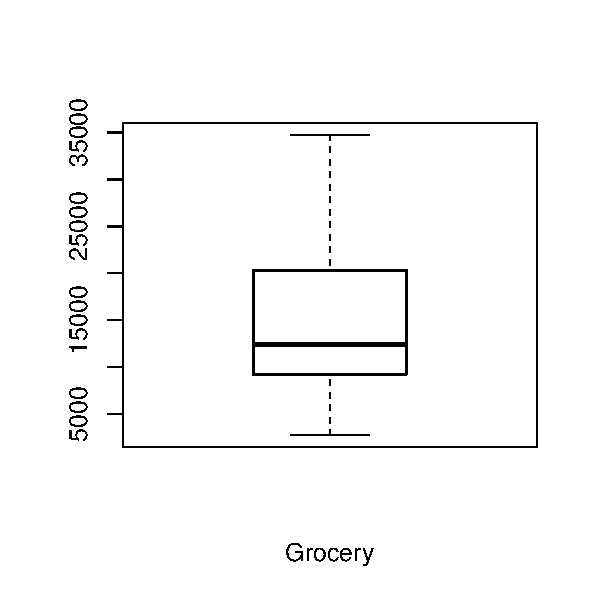
\includegraphics{7._K-means_Clustering_files/figure-latex/unnamed-chunk-16-1} \end{center}

Now, we'll deal with outliers for the \emph{Frozen} variable.

\begin{Shaded}
\begin{Highlighting}[]
\CommentTok{# sort all outliers of the Frozen variable}
\KeywordTok{sort}\NormalTok{(}\KeywordTok{boxplot.stats}\NormalTok{(retail.data}\OperatorTok{$}\NormalTok{Frozen)}\OperatorTok{$}\NormalTok{out)}
\end{Highlighting}
\end{Shaded}

\begin{verbatim}
## [1]  4736  5154  5612  5641  6746  7782  8132  8321 11559
\end{verbatim}

\begin{Shaded}
\begin{Highlighting}[]
\CommentTok{# examine percentiles of the Frozen variable higher than the 90th percentile}
\KeywordTok{quantile}\NormalTok{(retail.data}\OperatorTok{$}\NormalTok{Frozen, }\DataTypeTok{probs =} \KeywordTok{c}\NormalTok{(}\KeywordTok{seq}\NormalTok{(}\FloatTok{0.9}\NormalTok{, }\DecValTok{1}\NormalTok{, }\FloatTok{0.025}\NormalTok{)))}
\end{Highlighting}
\end{Shaded}

\begin{verbatim}
##      90%    92.5%      95%    97.5%     100% 
##  3519.50  4258.55  5133.10  7238.10 11559.00
\end{verbatim}

Setting values to the 92.5th percentile seem to be a good approach.

\begin{Shaded}
\begin{Highlighting}[]
\CommentTok{# store the 92.5th percentile of the Frozen variable to a new variable}
\NormalTok{new.max <-}\StringTok{ }\KeywordTok{as.numeric}\NormalTok{(}\KeywordTok{quantile}\NormalTok{(retail.data}\OperatorTok{$}\NormalTok{Frozen, }\DataTypeTok{probs =} \FloatTok{0.925}\NormalTok{))}

\CommentTok{# to all outliers of the Frozen variable assing the value of the 92.5th percentile}
\NormalTok{retail.data}\OperatorTok{$}\NormalTok{Frozen[retail.data}\OperatorTok{$}\NormalTok{Frozen }\OperatorTok{>}\StringTok{ }\NormalTok{new.max] <-}\StringTok{ }\NormalTok{new.max}

\CommentTok{# print a boxplot for the Frozen variable}
\KeywordTok{boxplot}\NormalTok{(retail.data}\OperatorTok{$}\NormalTok{Frozen, }\DataTypeTok{xlab=}\StringTok{'Frozen'}\NormalTok{)}
\end{Highlighting}
\end{Shaded}

\begin{center}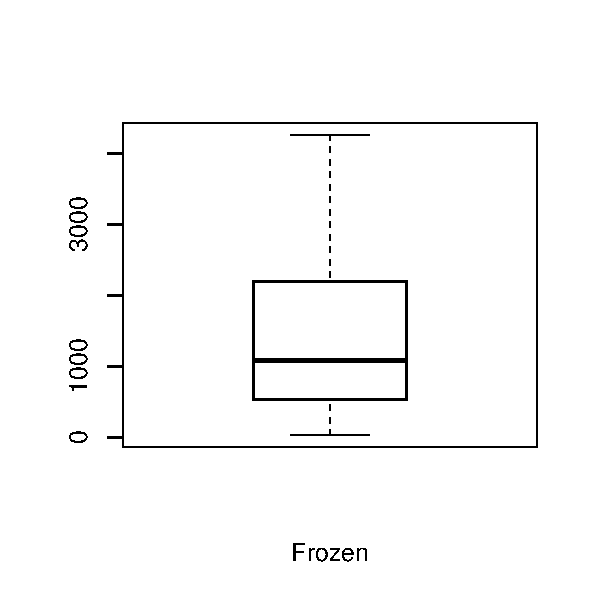
\includegraphics{7._K-means_Clustering_files/figure-latex/unnamed-chunk-18-1} \end{center}

Finally, examine the \emph{retail.data} after the transformations.

\begin{Shaded}
\begin{Highlighting}[]
\CommentTok{# print the sumary of the retail.data dataset}
\KeywordTok{summary}\NormalTok{(retail.data)}
\end{Highlighting}
\end{Shaded}

\begin{verbatim}
##           Region        Fresh            Milk          Grocery     
##  Lisbon      : 18   Min.   :   18   Min.   :  928   Min.   : 2743  
##  Oporto      : 19   1st Qu.: 2348   1st Qu.: 5938   1st Qu.: 9245  
##  Other_region:105   Median : 5994   Median : 7812   Median :12390  
##                     Mean   : 8460   Mean   : 9421   Mean   :15237  
##                     3rd Qu.:12230   3rd Qu.:12163   3rd Qu.:20184  
##                     Max.   :26287   Max.   :20638   Max.   :34732  
##      Frozen       Detergents_Paper  Delicatessen   
##  Min.   :  33.0   Min.   :  332    Min.   :   3.0  
##  1st Qu.: 534.2   1st Qu.: 3684    1st Qu.: 566.8  
##  Median :1081.0   Median : 5614    Median :1350.0  
##  Mean   :1471.9   Mean   : 6650    Mean   :1485.2  
##  3rd Qu.:2146.8   3rd Qu.: 8662    3rd Qu.:2156.0  
##  Max.   :4258.6   Max.   :16171    Max.   :3455.6
\end{verbatim}

\section{Clustering with 2 Features}\label{clustering-with-2-features}

Let's choose only two features for this initial, simple clustering. For
the sake of an example, let's pick Frozen and Milk variables.

\emph{NOTE:} We will choose only two features in order to demonstrate
the algorithm. But in reality, all numerical variables (that make sense)
should be taken into consideration.

\begin{Shaded}
\begin{Highlighting}[]
\CommentTok{# print the matrix of scatterplots for all numeric variables}
\KeywordTok{pairs}\NormalTok{(}\OperatorTok{~}\NormalTok{Fresh}\OperatorTok{+}\NormalTok{Frozen}\OperatorTok{+}\NormalTok{Grocery}\OperatorTok{+}\NormalTok{Milk}\OperatorTok{+}\NormalTok{Delicatessen}\OperatorTok{+}\NormalTok{Detergents_Paper, }\DataTypeTok{data =}\NormalTok{ retail.data)}
\end{Highlighting}
\end{Shaded}

\begin{center}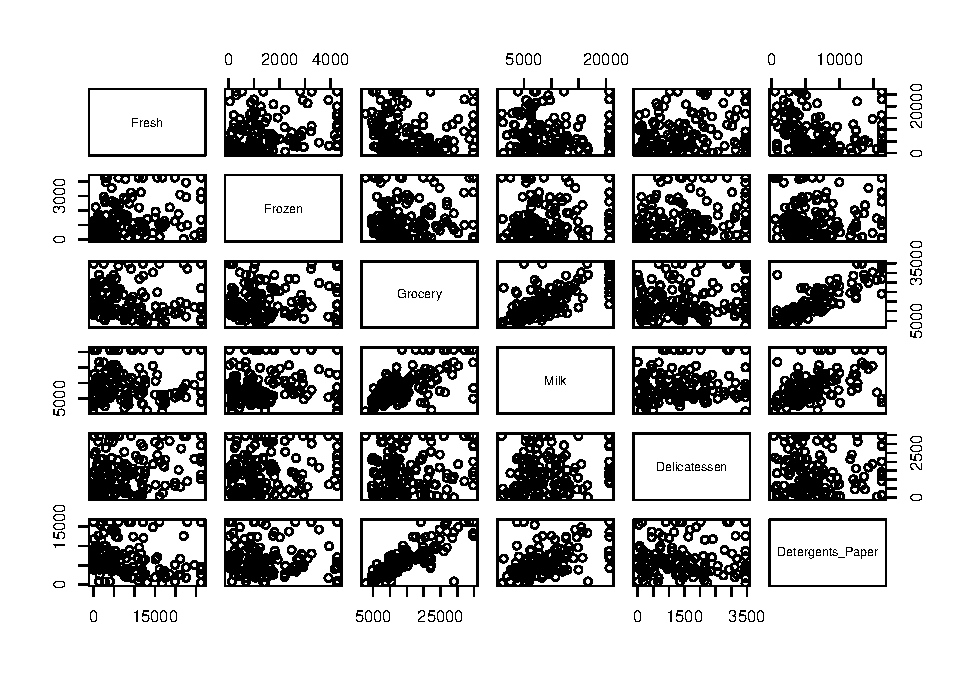
\includegraphics{7._K-means_Clustering_files/figure-latex/unnamed-chunk-20-1} \end{center}

By looking at the plots, no particular pattern can be observed. But for
the sake of an example, let's pick \emph{Frozen} and \emph{Milk}
variables. Get a closer look at selected variables.

\begin{Shaded}
\begin{Highlighting}[]
\CommentTok{# plot the scatterplot for the variablesFrozen and Milk}
\KeywordTok{ggplot}\NormalTok{(}\DataTypeTok{data=}\NormalTok{retail.data, }\KeywordTok{aes}\NormalTok{(}\DataTypeTok{x=}\NormalTok{Frozen, }\DataTypeTok{y=}\NormalTok{Milk)) }\OperatorTok{+}\StringTok{ }
\StringTok{  }\KeywordTok{geom_point}\NormalTok{(}\DataTypeTok{shape=}\DecValTok{1}\NormalTok{)}
\end{Highlighting}
\end{Shaded}

\begin{center}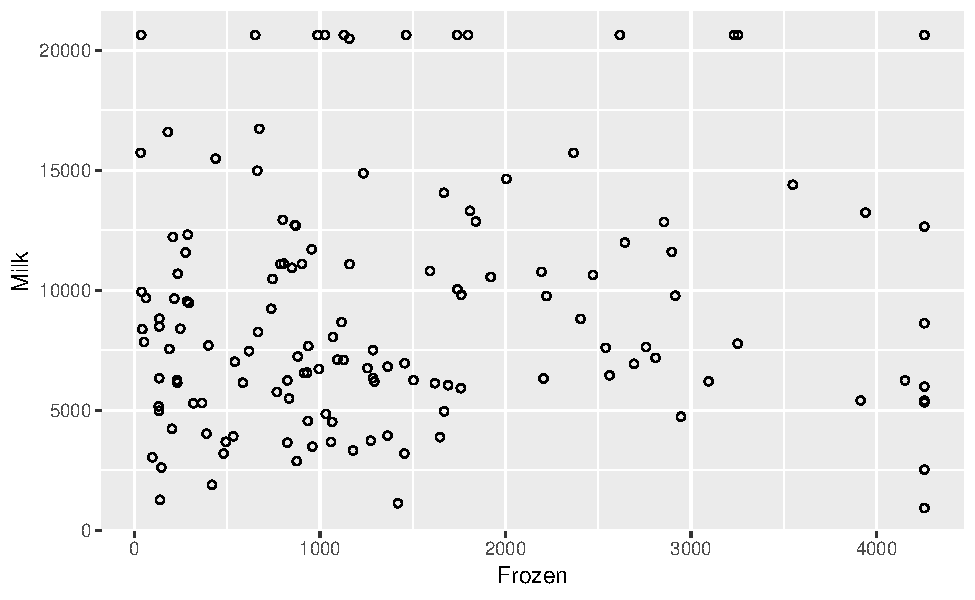
\includegraphics{7._K-means_Clustering_files/figure-latex/unnamed-chunk-21-1} \end{center}

No clear pattern in the data, but let's run K-means and see if some
clusters will emerge.

Create a subset of the original data containing the attributes to be
used in the K-means.

\begin{Shaded}
\begin{Highlighting}[]
\CommentTok{# create a subset of the data with variables Frozen and Milk}
\NormalTok{retail.data1 <-}\StringTok{ }\NormalTok{retail.data[, }\KeywordTok{c}\NormalTok{(}\StringTok{"Frozen"}\NormalTok{, }\StringTok{"Milk"}\NormalTok{)]}

\CommentTok{# print the summary of the new dataset}
\KeywordTok{summary}\NormalTok{(retail.data1)}
\end{Highlighting}
\end{Shaded}

\begin{verbatim}
##      Frozen            Milk      
##  Min.   :  33.0   Min.   :  928  
##  1st Qu.: 534.2   1st Qu.: 5938  
##  Median :1081.0   Median : 7812  
##  Mean   :1471.9   Mean   : 9421  
##  3rd Qu.:2146.8   3rd Qu.:12163  
##  Max.   :4258.6   Max.   :20638
\end{verbatim}

When variables are in incomparable units and/or the numeric values are
on very different scales of magnitude, they should be rescaled. Since
our variables Frozen and Milk have different value ranges, we need to
rescale the data. To that end, we will use normalization as there are no
outliers. Normalization is done using the formula:

\[Z = \frac{X - min(X)}{max(X) - min(X)}\]

Let's create q function for performing the normalization.

\begin{Shaded}
\begin{Highlighting}[]
\CommentTok{# function for performing the normalization}
\NormalTok{normalize.feature <-}\StringTok{ }\ControlFlowTok{function}\NormalTok{( feature ) \{}
  \ControlFlowTok{if}\NormalTok{ ( }\KeywordTok{sum}\NormalTok{(feature, }\DataTypeTok{na.rm =}\NormalTok{ T) }\OperatorTok{==}\StringTok{ }\DecValTok{0}\NormalTok{ ) feature}
  \ControlFlowTok{else}\NormalTok{ ((feature }\OperatorTok{-}\StringTok{ }\KeywordTok{min}\NormalTok{(feature, }\DataTypeTok{na.rm =}\NormalTok{ T))}\OperatorTok{/}\NormalTok{(}\KeywordTok{max}\NormalTok{(feature, }\DataTypeTok{na.rm =}\NormalTok{ T) }\OperatorTok{-}\StringTok{ }\KeywordTok{min}\NormalTok{(feature, }\DataTypeTok{na.rm =}\NormalTok{ T)))}
\NormalTok{\}}
\end{Highlighting}
\end{Shaded}

Then, we normalize all variables by calling our custom function
\emph{normalize.feature.}

\begin{Shaded}
\begin{Highlighting}[]
\CommentTok{# normalize both variables}
\NormalTok{retail.data1.norm <-}\StringTok{ }\KeywordTok{as.data.frame}\NormalTok{(}\KeywordTok{apply}\NormalTok{(retail.data1, }\DecValTok{2}\NormalTok{, normalize.feature))}

\CommentTok{# print the summary}
\KeywordTok{summary}\NormalTok{(retail.data1.norm)}
\end{Highlighting}
\end{Shaded}

\begin{verbatim}
##      Frozen            Milk       
##  Min.   :0.0000   Min.   :0.0000  
##  1st Qu.:0.1186   1st Qu.:0.2542  
##  Median :0.2480   Median :0.3493  
##  Mean   :0.3405   Mean   :0.4309  
##  3rd Qu.:0.5002   3rd Qu.:0.5700  
##  Max.   :1.0000   Max.   :1.0000
\end{verbatim}

Run the K Means algorithm, specifying, for example, 4 centers.
\emph{`iter.max'} defines the maximum number of iterations. This
overcomes the problem of situations where there is a slow convergence.
This clustering approach can be sensitive to the initial selection of
centroids. \emph{`nstart'} option attempts multiple initial
configurations and reports on the best one. Afterward, we inspect the
results.

\begin{Shaded}
\begin{Highlighting}[]
\CommentTok{# set the seed}
\KeywordTok{set.seed}\NormalTok{(}\DecValTok{3108}\NormalTok{)}

\CommentTok{# run the clustering with 4 clusters, iter.max=20, nstart=1000}
\NormalTok{simple.4k <-}\StringTok{ }\KeywordTok{kmeans}\NormalTok{(}\DataTypeTok{x =}\NormalTok{ retail.data1.norm, }\DataTypeTok{centers=}\DecValTok{4}\NormalTok{, }\DataTypeTok{iter.max=}\DecValTok{20}\NormalTok{, }\DataTypeTok{nstart=}\DecValTok{1000}\NormalTok{)}

\CommentTok{# print the model}
\NormalTok{simple.4k}
\end{Highlighting}
\end{Shaded}

\begin{verbatim}
## K-means clustering with 4 clusters of sizes 10, 35, 72, 25
## 
## Cluster means:
##      Frozen      Milk
## 1 0.8887541 0.8903003
## 2 0.2417335 0.7118702
## 3 0.1734192 0.2642975
## 4 0.7407727 0.3335116
## 
## Clustering vector:
##   1   2   3   5   6   7   8  10  11  12  13  14  15  17  19  21  24  25 
##   3   3   4   4   3   3   3   2   4   3   2   4   3   3   4   3   1   4 
##  26  29  36  38  39  43  44  45  46  47  48  49  50  53  54  57  58  61 
##   3   2   3   2   2   3   2   3   2   2   1   3   2   3   3   1   3   3 
##  62  63  64  66  68  74  75  78  82  83  85  86  87  93  95  97 101 102 
##   1   4   4   2   3   4   3   2   3   3   3   2   2   1   2   3   4   2 
## 103 107 108 109 110 112 124 128 146 156 157 159 160 161 164 165 166 167 
##   4   3   4   3   2   2   4   3   3   3   3   3   3   3   2   4   1   3 
## 171 172 174 176 189 190 194 198 201 202 206 208 210 212 215 217 219 224 
##   3   2   3   3   4   2   3   3   1   1   2   4   2   1   3   2   3   4 
## 227 231 246 252 265 267 269 280 282 294 296 298 299 301 302 303 304 305 
##   3   4   3   1   3   4   3   3   3   2   3   3   3   3   2   3   3   3 
## 306 307 310 313 316 320 332 334 335 336 341 342 344 347 348 350 352 354 
##   2   2   2   3   2   2   2   3   4   3   3   3   3   4   4   2   2   3 
## 358 366 371 374 377 380 397 408 409 416 417 419 422 424 425 438 
##   3   3   3   3   4   3   4   4   3   3   2   3   3   3   3   2 
## 
## Within cluster sum of squares by cluster:
## [1] 0.4615838 1.9864552 2.0309120 1.3114720
##  (between_SS / total_SS =  74.0 %)
## 
## Available components:
## 
## [1] "cluster"      "centers"      "totss"        "withinss"    
## [5] "tot.withinss" "betweenss"    "size"         "iter"        
## [9] "ifault"
\end{verbatim}

From the output, we can observe the following evaluation metrics:

\begin{itemize}
\item
  \textbf{within\_SS (within-cluster sum of squares)}: The sum of
  squared differences between individual data points in a cluster and
  the cluster center (centroid). It is computed for each cluster;
\item
  \textbf{total\_SS (total sum of squares)}: The sum of squared
  differences of each data point to the global sample mean;
\item
  \textbf{between\_SS (between cluster sum of squares)}: The sum of
  squared differences of each centroid to the global sample mean (when
  computing this value, the squared difference of each cluster center to
  the global sample mean is multiplied by the number of data points in
  that cluster);
\item
  \textbf{between\_SS / total\_SS}: This ratio indicates how `well' the
  sample splits into clusters; the higher the ratio, the better the
  clustering. The maximum is 1.
\end{itemize}

Add the vector of clusters to the data frame as a new variable
\emph{`cluster'} and plot it.

\begin{Shaded}
\begin{Highlighting}[]
\CommentTok{# add the cluster as a new variable to the dataset}
\NormalTok{retail.data1.norm}\OperatorTok{$}\NormalTok{cluster <-}\StringTok{ }\KeywordTok{factor}\NormalTok{(simple.4k}\OperatorTok{$}\NormalTok{cluster)}

\CommentTok{# print several instances of the dataset}
\KeywordTok{head}\NormalTok{(retail.data1.norm)}
\end{Highlighting}
\end{Shaded}

\begin{verbatim}
##       Frozen      Milk cluster
## 1 0.04283466 0.4428231       3
## 2 0.40917750 0.4506365       3
## 3 0.56134704 0.3997991       4
## 5 0.91869697 0.2273984       4
## 6 0.14980298 0.3719451       3
## 7 0.10578505 0.1152213       3
\end{verbatim}

Let's plot the data and new centroids.

\begin{Shaded}
\begin{Highlighting}[]
\CommentTok{# plot the clusters along with their centroids and color the points by their respective clusters}
\KeywordTok{ggplot}\NormalTok{(}\DataTypeTok{data=}\NormalTok{retail.data1.norm, }\KeywordTok{aes}\NormalTok{(}\DataTypeTok{x=}\NormalTok{Frozen, }\DataTypeTok{y=}\NormalTok{Milk, }\DataTypeTok{colour=}\NormalTok{cluster)) }\OperatorTok{+}\StringTok{ }
\StringTok{  }\KeywordTok{geom_point}\NormalTok{() }\OperatorTok{+}\StringTok{ }
\StringTok{  }\KeywordTok{xlab}\NormalTok{(}\StringTok{"Annual spending on frozen products"}\NormalTok{) }\OperatorTok{+}\StringTok{ }
\StringTok{  }\KeywordTok{ylab}\NormalTok{(}\StringTok{"Annual spending on dairy products"}\NormalTok{) }\OperatorTok{+}\StringTok{ }
\StringTok{  }\KeywordTok{ggtitle}\NormalTok{(}\StringTok{"Retail customers annual spending"}\NormalTok{) }\OperatorTok{+}\StringTok{ }
\StringTok{  }\CommentTok{# add cluster centers}
\StringTok{  }\KeywordTok{geom_point}\NormalTok{(}\DataTypeTok{data=}\KeywordTok{as.data.frame}\NormalTok{(simple.4k}\OperatorTok{$}\NormalTok{centers), }\DataTypeTok{colour=}\StringTok{"black"}\NormalTok{, }\DataTypeTok{size=}\DecValTok{4}\NormalTok{, }\DataTypeTok{shape=}\DecValTok{17}\NormalTok{) }
\end{Highlighting}
\end{Shaded}

\begin{center}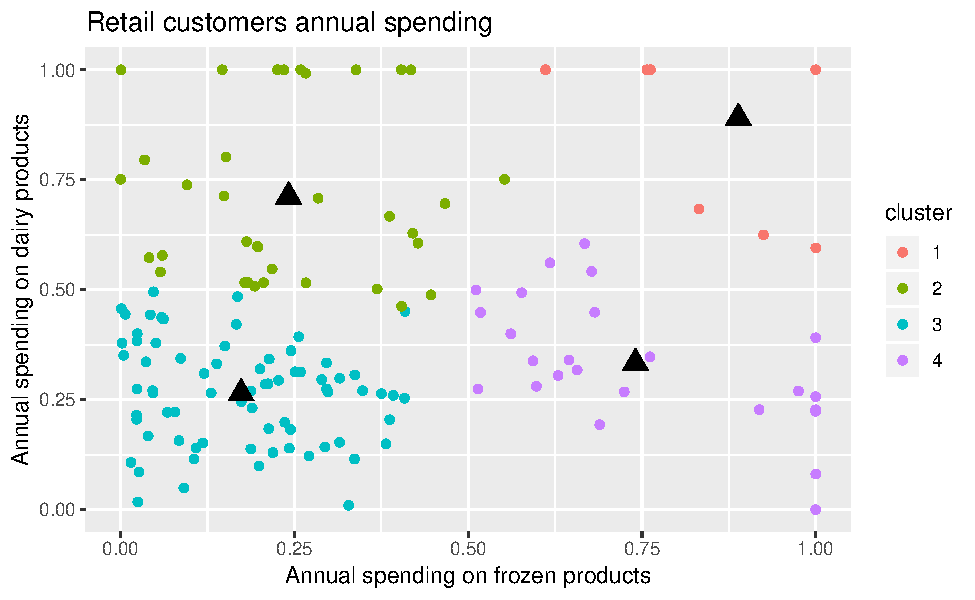
\includegraphics{7._K-means_Clustering_files/figure-latex/unnamed-chunk-27-1} \end{center}

The plot allows us to visually inspect the clusters, but it is better to
have a more systematic approach to judging the quality of clustering and
selecting the best value for K.

\section{Selecting the Best Value for
K}\label{selecting-the-best-value-for-k}

\subsection{Selection based on the Elbow
Method}\label{selection-based-on-the-elbow-method}

Instead of guessing the correct value for K, we can take a more
systematic approach to choose the `right' K. It is called the
\textbf{Elbow method}, and is based on the sum of squared differences
between data points and cluster centers, that is, the sum of
\emph{within\_SS} for all the clusters (tot.withinss).

Let us run the K-means for different values for K (from 2 to 8). We will
compute the metric required for the Elbow method (tot.withinss). Along
the way, we'll also compute the other metric: \emph{ratio of between\_SS
and total\_SS}.

\begin{Shaded}
\begin{Highlighting}[]
\CommentTok{# create an empty data frame}
\NormalTok{eval.metrics.2var <-}\StringTok{ }\KeywordTok{data.frame}\NormalTok{()}

\CommentTok{# remove the column with clusters}
\NormalTok{retail.data1.norm}\OperatorTok{$}\NormalTok{cluster <-}\StringTok{ }\OtherTok{NULL}

\CommentTok{# run kmeans for all K values in the range 2:8}
\ControlFlowTok{for}\NormalTok{ (k }\ControlFlowTok{in} \DecValTok{2}\OperatorTok{:}\DecValTok{8}\NormalTok{) \{}
  \KeywordTok{set.seed}\NormalTok{(}\DecValTok{3108}\NormalTok{)}
\NormalTok{  km.res <-}\StringTok{ }\KeywordTok{kmeans}\NormalTok{(}\DataTypeTok{x=}\NormalTok{retail.data1.norm, }\DataTypeTok{centers=}\NormalTok{k, }\DataTypeTok{iter.max=}\DecValTok{20}\NormalTok{, }\DataTypeTok{nstart =} \DecValTok{1000}\NormalTok{)}
  \CommentTok{# combine cluster number and the error measure, write to df}
\NormalTok{  eval.metrics.2var <-}\StringTok{ }\KeywordTok{rbind}\NormalTok{(eval.metrics.2var, }
                             \KeywordTok{c}\NormalTok{(k, km.res}\OperatorTok{$}\NormalTok{tot.withinss, km.res}\OperatorTok{$}\NormalTok{betweenss}\OperatorTok{/}\NormalTok{km.res}\OperatorTok{$}\NormalTok{totss)) }
\NormalTok{\}}

\CommentTok{# update the column names}
\KeywordTok{names}\NormalTok{(eval.metrics.2var) <-}\StringTok{ }\KeywordTok{c}\NormalTok{(}\StringTok{"cluster"}\NormalTok{, }\StringTok{"tot.within.ss"}\NormalTok{, }\StringTok{"ratio"}\NormalTok{)}

\CommentTok{# print the metrics}
\NormalTok{eval.metrics.2var}
\end{Highlighting}
\end{Shaded}

\begin{verbatim}
##   cluster tot.within.ss     ratio
## 1       2     12.577765 0.4350165
## 2       3      7.981614 0.6414721
## 3       4      5.790423 0.7398987
## 4       5      4.538501 0.7961340
## 5       6      3.368527 0.8486884
## 6       7      2.815509 0.8735295
## 7       8      2.374140 0.8933555
\end{verbatim}

Draw the Elbow plot.

\begin{Shaded}
\begin{Highlighting}[]
\CommentTok{# plot the line chart for cluster vs. tot.within.ss }
\KeywordTok{ggplot}\NormalTok{(}\DataTypeTok{data=}\NormalTok{eval.metrics.2var, }\KeywordTok{aes}\NormalTok{(}\DataTypeTok{x=}\NormalTok{cluster, }\DataTypeTok{y=}\NormalTok{tot.within.ss)) }\OperatorTok{+}\StringTok{ }
\StringTok{  }\KeywordTok{geom_line}\NormalTok{() }\OperatorTok{+}
\StringTok{  }\KeywordTok{ggtitle}\NormalTok{(}\StringTok{"Reduction in error for different values of K}\CharTok{\textbackslash{}n}\StringTok{"}\NormalTok{) }\OperatorTok{+}
\StringTok{  }\KeywordTok{xlab}\NormalTok{(}\StringTok{"}\CharTok{\textbackslash{}n}\StringTok{Clusters"}\NormalTok{) }\OperatorTok{+}\StringTok{ }
\StringTok{  }\KeywordTok{ylab}\NormalTok{(}\StringTok{"Total Within Cluster Sum of Squares}\CharTok{\textbackslash{}n}\StringTok{"}\NormalTok{) }\OperatorTok{+}
\StringTok{  }\KeywordTok{scale_x_continuous}\NormalTok{(}\DataTypeTok{breaks=}\KeywordTok{seq}\NormalTok{(}\DataTypeTok{from=}\DecValTok{0}\NormalTok{, }\DataTypeTok{to=}\DecValTok{8}\NormalTok{, }\DataTypeTok{by=}\DecValTok{1}\NormalTok{))}
\end{Highlighting}
\end{Shaded}

\begin{center}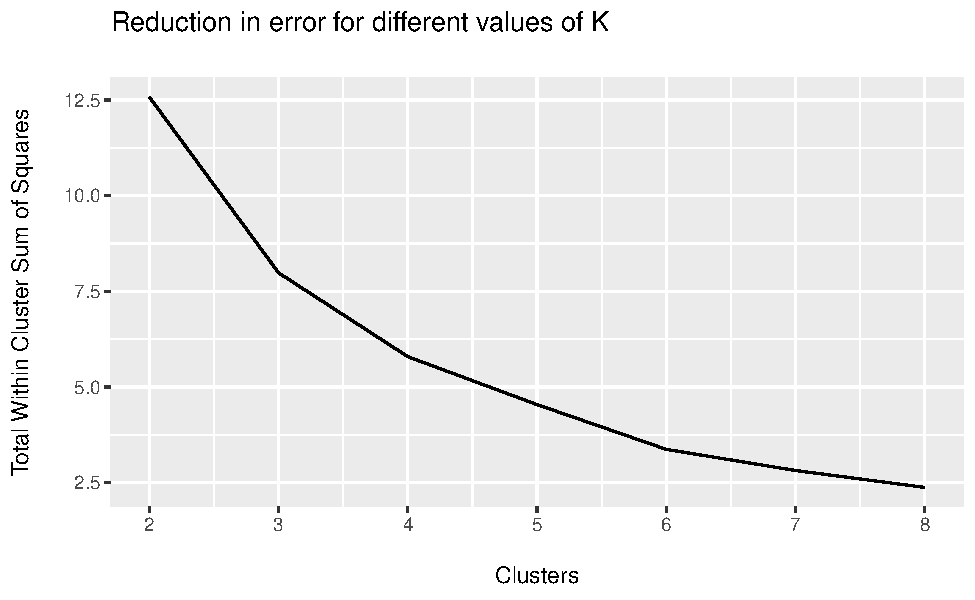
\includegraphics{7._K-means_Clustering_files/figure-latex/unnamed-chunk-29-1} \end{center}

It seems that \emph{K=3} or \emph{K=4} would be the best options for the
number of clusters.

If it is not fully clear from the plot where we have a significant
decrease in the \emph{tot.within.ss} value, we can compute the
difference between every two subsequent values. We will load the file
with our utility functions (code is given at the end of the script) and
call our custom function \emph{compute.difference}.

\begin{Shaded}
\begin{Highlighting}[]
\CommentTok{# load the source code from the Utility.R file}
\KeywordTok{source}\NormalTok{(}\StringTok{"Utility.R"}\NormalTok{)}

\CommentTok{# calculate the ratio difference for different K values (from 2 to 8) }
\KeywordTok{data.frame}\NormalTok{(}\DataTypeTok{K=}\DecValTok{2}\OperatorTok{:}\DecValTok{8}\NormalTok{, }
           \DataTypeTok{tot.within.ss.delta=}\KeywordTok{compute.difference}\NormalTok{(eval.metrics.2var}\OperatorTok{$}\NormalTok{tot.within.ss),}
           \DataTypeTok{ratio.delta=}\KeywordTok{compute.difference}\NormalTok{(eval.metrics.2var}\OperatorTok{$}\NormalTok{ratio))}
\end{Highlighting}
\end{Shaded}

\begin{verbatim}
##   K tot.within.ss.delta ratio.delta
## 1 2                  NA          NA
## 2 3           4.5961507  0.20645554
## 3 4           2.1911907  0.09842659
## 4 5           1.2519218  0.05623536
## 5 6           1.1699738  0.05255432
## 6 7           0.5530184  0.02484116
## 7 8           0.4413690  0.01982595
\end{verbatim}

As we've already examined the solution with 4 clusters, let's also
examine the solution with K=3.

\begin{Shaded}
\begin{Highlighting}[]
\CommentTok{# set the seed value}
\KeywordTok{set.seed}\NormalTok{(}\DecValTok{3108}\NormalTok{)}

\CommentTok{# run the clustering for 3 clusters, iter.max=20, nstart=1000}
\NormalTok{simple.3k <-}\StringTok{ }\KeywordTok{kmeans}\NormalTok{(}\DataTypeTok{x =}\NormalTok{ retail.data1.norm, }\DataTypeTok{centers=}\DecValTok{3}\NormalTok{, }\DataTypeTok{iter.max=}\DecValTok{20}\NormalTok{, }\DataTypeTok{nstart=}\DecValTok{1000}\NormalTok{)}

\CommentTok{# store the (factorized) cluster value in a new variable }
\NormalTok{retail.data1.norm}\OperatorTok{$}\NormalTok{cluster <-}\StringTok{ }\KeywordTok{factor}\NormalTok{(simple.3k}\OperatorTok{$}\NormalTok{cluster)}
\end{Highlighting}
\end{Shaded}

Plot the 3-cluster solution.

\begin{Shaded}
\begin{Highlighting}[]
\CommentTok{# plot the clusters along with their centroids}
\KeywordTok{ggplot}\NormalTok{(}\DataTypeTok{data=}\NormalTok{retail.data1.norm, }\KeywordTok{aes}\NormalTok{(}\DataTypeTok{x=}\NormalTok{Frozen, }\DataTypeTok{y=}\NormalTok{Milk, }\DataTypeTok{colour=}\NormalTok{cluster)) }\OperatorTok{+}\StringTok{ }
\StringTok{    }\KeywordTok{geom_point}\NormalTok{() }\OperatorTok{+}
\StringTok{    }\KeywordTok{xlab}\NormalTok{(}\StringTok{"Annual spending on frozen products"}\NormalTok{) }\OperatorTok{+}
\StringTok{    }\KeywordTok{ylab}\NormalTok{(}\StringTok{"Annual spending on dairy products"}\NormalTok{) }\OperatorTok{+}
\StringTok{    }\KeywordTok{ggtitle}\NormalTok{(}\StringTok{"Retail customers annual spending"}\NormalTok{) }\OperatorTok{+}
\StringTok{    }\KeywordTok{geom_point}\NormalTok{(}\DataTypeTok{data=}\KeywordTok{as.data.frame}\NormalTok{(simple.3k}\OperatorTok{$}\NormalTok{centers),}
                     \DataTypeTok{colour=}\StringTok{"black"}\NormalTok{,}\DataTypeTok{size=}\DecValTok{4}\NormalTok{, }\DataTypeTok{shape=}\DecValTok{17}\NormalTok{)}
\end{Highlighting}
\end{Shaded}

\begin{center}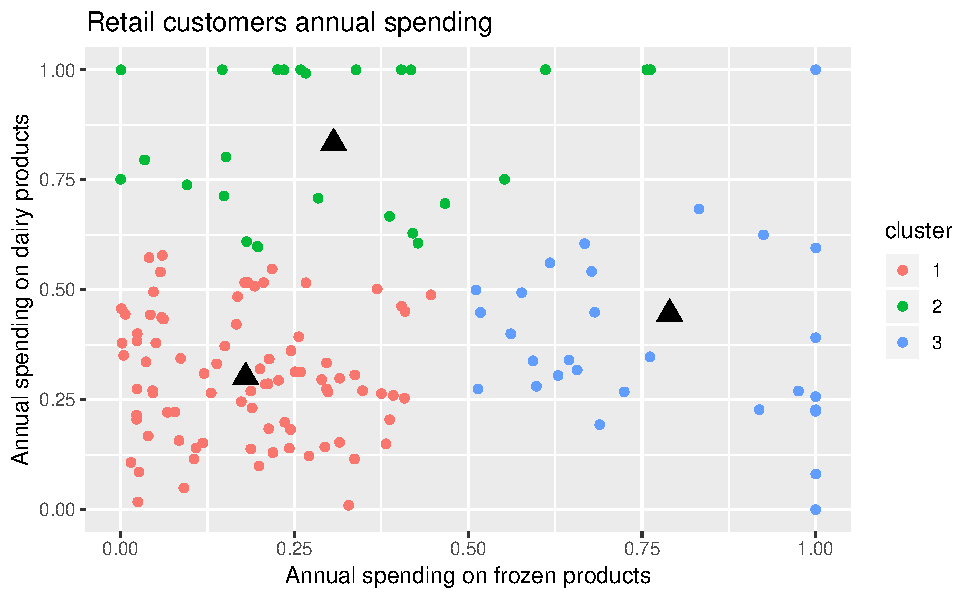
\includegraphics{7._K-means_Clustering_files/figure-latex/unnamed-chunk-32-1} \end{center}

Next, we examine clusters closer by looking into the cluster centers
(mean) and standard deviation from the centers. When examining clusters
- in order to interpret them - we use `regular' (not normalized)
features. The \emph{summary.stats()} f. used below is a custom function
defined in the \emph{Utility.R}.

\begin{Shaded}
\begin{Highlighting}[]
\CommentTok{# calculate the mean and sd values for all three clusters }
\NormalTok{sum.stats <-}\StringTok{ }\KeywordTok{summary.stats}\NormalTok{(}\DataTypeTok{feature.set =}\NormalTok{ retail.data1, }
                           \DataTypeTok{clusters =}\NormalTok{ simple.3k}\OperatorTok{$}\NormalTok{cluster, }
                           \DataTypeTok{cl.num =} \DecValTok{3}\NormalTok{)}

\NormalTok{sum.stats}
\end{Highlighting}
\end{Shaded}

\begin{verbatim}
##   attributes         Mean (SD)          Mean (SD)         Mean (SD)
## 1    cluster                 1                  2                 3
## 2       freq                84                 26                32
## 3     Frozen   793.04 (526.94)   1328.08 (879.37)  3370.69 (797.97)
## 4       Milk 6862.69 (2782.19) 17342.03 (3268.35) 9699.39 (5204.43)
\end{verbatim}

The solution with \textbf{K=4} seems to be better as features are less
dispersed than here (e.g.~the \emph{Milk} variable in cluster 3, and
\emph{Frozen} variable in cluster 2 have very high dispersion). The
solution with \textbf{K=4} resolves this (check the plot and examine
cluster centers).

\section{Clustering with All Numeric
Features}\label{clustering-with-all-numeric-features}

Since the 6 numeric attributes differ in their value ranges, we need to
normalize them, that is, transform them to the value range {[}0,1{]}.

\begin{Shaded}
\begin{Highlighting}[]
\CommentTok{# normalize all numeric variables from the retail.data dataset}
\NormalTok{retail.norm <-}\StringTok{ }\KeywordTok{as.data.frame}\NormalTok{(}\KeywordTok{apply}\NormalTok{(retail.data[,}\KeywordTok{c}\NormalTok{(}\DecValTok{2}\OperatorTok{:}\DecValTok{7}\NormalTok{)], }\DecValTok{2}\NormalTok{, normalize.feature))}

\CommentTok{# print the summary}
\KeywordTok{summary}\NormalTok{(retail.norm)}
\end{Highlighting}
\end{Shaded}

\begin{verbatim}
##      Fresh              Milk           Grocery           Frozen      
##  Min.   :0.00000   Min.   :0.0000   Min.   :0.0000   Min.   :0.0000  
##  1st Qu.:0.08869   1st Qu.:0.2542   1st Qu.:0.2033   1st Qu.:0.1186  
##  Median :0.22747   Median :0.3493   Median :0.3016   Median :0.2480  
##  Mean   :0.32138   Mean   :0.4309   Mean   :0.3906   Mean   :0.3405  
##  3rd Qu.:0.46487   3rd Qu.:0.5700   3rd Qu.:0.5452   3rd Qu.:0.5002  
##  Max.   :1.00000   Max.   :1.0000   Max.   :1.0000   Max.   :1.0000  
##  Detergents_Paper  Delicatessen   
##  Min.   :0.0000   Min.   :0.0000  
##  1st Qu.:0.2116   1st Qu.:0.1633  
##  Median :0.3335   Median :0.3901  
##  Mean   :0.3989   Mean   :0.4293  
##  3rd Qu.:0.5260   3rd Qu.:0.6236  
##  Max.   :1.0000   Max.   :1.0000
\end{verbatim}

Instead of guessing K, we'll right away use the Elbow method to find the
optimal value for K.

\begin{Shaded}
\begin{Highlighting}[]
\CommentTok{# create an empty data frame}
\NormalTok{eval.metrics.6var <-}\StringTok{ }\KeywordTok{data.frame}\NormalTok{()}

\CommentTok{# run kmeans for all K values in the range 2:8}
\ControlFlowTok{for}\NormalTok{ (k }\ControlFlowTok{in} \DecValTok{2}\OperatorTok{:}\DecValTok{8}\NormalTok{) \{}
  \KeywordTok{set.seed}\NormalTok{(}\DecValTok{3108}\NormalTok{)}
\NormalTok{  km.res <-}\StringTok{ }\KeywordTok{kmeans}\NormalTok{(}\DataTypeTok{x=}\NormalTok{retail.norm, }\DataTypeTok{centers=}\NormalTok{k, }\DataTypeTok{iter.max=}\DecValTok{20}\NormalTok{, }\DataTypeTok{nstart =} \DecValTok{1000}\NormalTok{)}
  \CommentTok{# combine cluster number and the error measure, write to df}
\NormalTok{  eval.metrics.6var <-}\StringTok{ }\KeywordTok{rbind}\NormalTok{(eval.metrics.6var, }
                             \KeywordTok{c}\NormalTok{(k, km.res}\OperatorTok{$}\NormalTok{tot.withinss, km.res}\OperatorTok{$}\NormalTok{betweenss}\OperatorTok{/}\NormalTok{km.res}\OperatorTok{$}\NormalTok{totss)) }
\NormalTok{\}}

\CommentTok{# update the column names}
\KeywordTok{names}\NormalTok{(eval.metrics.6var) <-}\StringTok{ }\KeywordTok{c}\NormalTok{(}\StringTok{"cluster"}\NormalTok{, }\StringTok{"tot.within.ss"}\NormalTok{, }\StringTok{"ratio"}\NormalTok{)}
\NormalTok{eval.metrics.6var}
\end{Highlighting}
\end{Shaded}

\begin{verbatim}
##   cluster tot.within.ss     ratio
## 1       2      49.72071 0.2667494
## 2       3      39.96778 0.4105797
## 3       4      35.23843 0.4803252
## 4       5      31.13015 0.5409116
## 5       6      27.49447 0.5945284
## 6       7      25.18087 0.6286479
## 7       8      23.36426 0.6554381
\end{verbatim}

Draw the Elbow plot.

\begin{Shaded}
\begin{Highlighting}[]
\CommentTok{# plot the clusters along with their centroids}
\KeywordTok{ggplot}\NormalTok{(}\DataTypeTok{data=}\NormalTok{eval.metrics.6var, }\KeywordTok{aes}\NormalTok{(}\DataTypeTok{x=}\NormalTok{cluster, }\DataTypeTok{y=}\NormalTok{tot.within.ss)) }\OperatorTok{+}\StringTok{ }
\StringTok{  }\KeywordTok{geom_line}\NormalTok{() }\OperatorTok{+}
\StringTok{  }\KeywordTok{ggtitle}\NormalTok{(}\StringTok{"Reduction in error for different values of K}\CharTok{\textbackslash{}n}\StringTok{"}\NormalTok{) }\OperatorTok{+}
\StringTok{  }\KeywordTok{xlab}\NormalTok{(}\StringTok{"}\CharTok{\textbackslash{}n}\StringTok{Clusters"}\NormalTok{) }\OperatorTok{+}\StringTok{ }
\StringTok{  }\KeywordTok{ylab}\NormalTok{(}\StringTok{"Total Within Cluster Sum of Squares}\CharTok{\textbackslash{}n}\StringTok{"}\NormalTok{) }\OperatorTok{+}
\StringTok{  }\KeywordTok{scale_x_continuous}\NormalTok{(}\DataTypeTok{breaks=}\KeywordTok{seq}\NormalTok{(}\DataTypeTok{from=}\DecValTok{0}\NormalTok{, }\DataTypeTok{to=}\DecValTok{8}\NormalTok{, }\DataTypeTok{by=}\DecValTok{1}\NormalTok{))}
\end{Highlighting}
\end{Shaded}

\begin{center}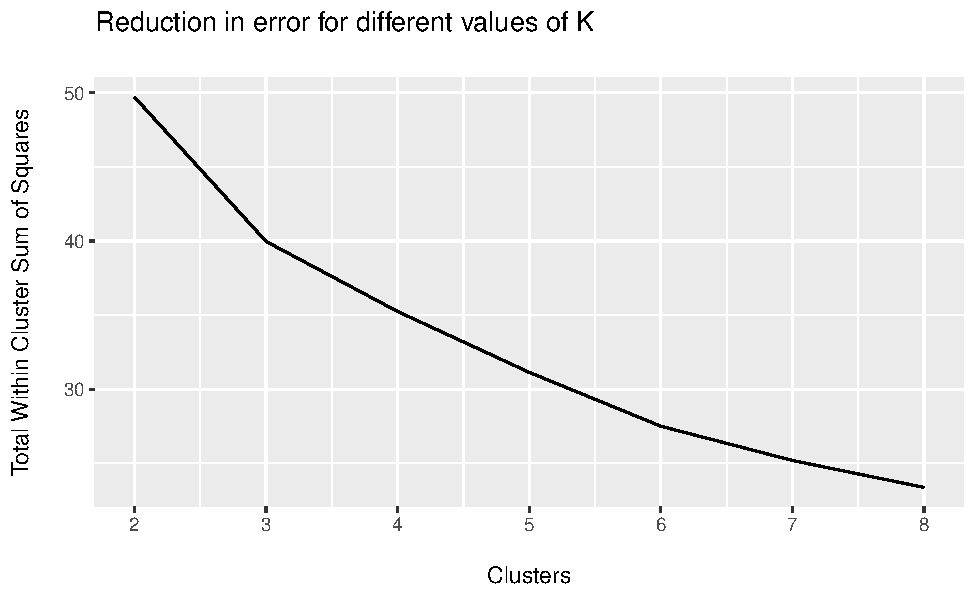
\includegraphics{7._K-means_Clustering_files/figure-latex/unnamed-chunk-36-1} \end{center}

This time it seems that the solution with 3 clusters might be the best.

As previously done, we'll also look for the best value for K by
examining the difference between every two subsequent values of
tot.within.ss and ratio (of \emph{between.SS} and \emph{total.SS}).

\begin{Shaded}
\begin{Highlighting}[]
\CommentTok{# calculate the ratio difference for different K values (from 2 to 8) }
\KeywordTok{data.frame}\NormalTok{(}\DataTypeTok{k=}\KeywordTok{c}\NormalTok{(}\DecValTok{2}\OperatorTok{:}\DecValTok{8}\NormalTok{),}
           \DataTypeTok{tot.within.ss.delta=}\KeywordTok{compute.difference}\NormalTok{(eval.metrics.6var}\OperatorTok{$}\NormalTok{tot.within.ss),}
           \DataTypeTok{ration.delta=}\KeywordTok{compute.difference}\NormalTok{(eval.metrics.6var}\OperatorTok{$}\NormalTok{ratio))}
\end{Highlighting}
\end{Shaded}

\begin{verbatim}
##   k tot.within.ss.delta ration.delta
## 1 2                  NA           NA
## 2 3            9.752931   0.14383025
## 3 4            4.729349   0.06974554
## 4 5            4.108280   0.06058640
## 5 6            3.635680   0.05361679
## 6 7            2.313597   0.03411951
## 7 8            1.816606   0.02679019
\end{verbatim}

This again suggests 3 clusters as the best option.

Let's examine in detail clustering with K=3.

\begin{Shaded}
\begin{Highlighting}[]
\CommentTok{# set the seed}
\KeywordTok{set.seed}\NormalTok{(}\DecValTok{3108}\NormalTok{)}

\CommentTok{# run the clustering for 3 clusters, iter.max=20, nstart=1000}
\NormalTok{retail.3k.6var <-}\StringTok{ }\KeywordTok{kmeans}\NormalTok{(}\DataTypeTok{x=}\NormalTok{retail.norm, }\DataTypeTok{centers=}\DecValTok{3}\NormalTok{, }\DataTypeTok{iter.max=}\DecValTok{20}\NormalTok{, }\DataTypeTok{nstart =} \DecValTok{1000}\NormalTok{)}

\CommentTok{# examine cluster centers}
\NormalTok{sum.stats <-}\StringTok{ }\KeywordTok{summary.stats}\NormalTok{(}\DataTypeTok{feature.set =}\NormalTok{ retail.norm, }\CommentTok{#retail.data[,c(2:7)], }
                           \DataTypeTok{clusters =}\NormalTok{ retail.3k.6var}\OperatorTok{$}\NormalTok{cluster, }
                           \DataTypeTok{cl.num =} \DecValTok{3}\NormalTok{)}
\NormalTok{sum.stats}
\end{Highlighting}
\end{Shaded}

\begin{verbatim}
##         attributes   Mean (SD)   Mean (SD)   Mean (SD)
## 1          cluster           1           2           3
## 2             freq          43          25          74
## 3            Fresh 0.55 (0.31)  0.36 (0.3) 0.18 (0.17)
## 4             Milk 0.32 (0.18) 0.83 (0.23) 0.36 (0.19)
## 5          Grocery 0.22 (0.13) 0.81 (0.18) 0.34 (0.18)
## 6           Frozen  0.5 (0.32) 0.44 (0.34) 0.21 (0.19)
## 7 Detergents_Paper  0.2 (0.12) 0.83 (0.18) 0.37 (0.19)
## 8     Delicatessen 0.63 (0.27) 0.59 (0.33) 0.26 (0.22)
\end{verbatim}

\section{\texorpdfstring{Appendix: Utility Functions (`Utility.R'
file)}{Appendix: Utility Functions (Utility.R file)}}\label{appendix-utility-functions-utility.r-file}

\begin{Shaded}
\begin{Highlighting}[]
\NormalTok{## function that computes the difference between two consecutive values}
\NormalTok{compute.difference <-}\StringTok{ }\ControlFlowTok{function}\NormalTok{(values) \{}
\NormalTok{  dif <-}\StringTok{ }\KeywordTok{vector}\NormalTok{(}\DataTypeTok{mode =} \StringTok{"numeric"}\NormalTok{, }\DataTypeTok{length =} \KeywordTok{length}\NormalTok{(values))}
\NormalTok{  dif[}\DecValTok{1}\NormalTok{] <-}\StringTok{ }\OtherTok{NA}
  \ControlFlowTok{for}\NormalTok{(i }\ControlFlowTok{in} \DecValTok{1}\OperatorTok{:}\NormalTok{(}\KeywordTok{length}\NormalTok{(values)}\OperatorTok{-}\DecValTok{1}\NormalTok{)) \{}
\NormalTok{    dif[i}\OperatorTok{+}\DecValTok{1}\NormalTok{] <-}\StringTok{ }\KeywordTok{abs}\NormalTok{(values[i}\OperatorTok{+}\DecValTok{1}\NormalTok{] }\OperatorTok{-}\StringTok{ }\NormalTok{values[i])}
\NormalTok{  \}}
\NormalTok{  dif}
\NormalTok{\}}

\NormalTok{## function that provides summary statistics about clusters}
\NormalTok{summary.stats <-}\StringTok{ }\ControlFlowTok{function}\NormalTok{(feature.set, clusters, cl.num) \{}
\NormalTok{  sum.stats <-}\StringTok{ }\KeywordTok{aggregate}\NormalTok{(}\DataTypeTok{x =}\NormalTok{ feature.set, }
                         \DataTypeTok{by =} \KeywordTok{list}\NormalTok{(clusters), }
                         \DataTypeTok{FUN =} \ControlFlowTok{function}\NormalTok{(x) \{ }
\NormalTok{                           m <-}\StringTok{ }\KeywordTok{mean}\NormalTok{(x, }\DataTypeTok{na.rm =}\NormalTok{ T)}
\NormalTok{                           sd <-}\StringTok{ }\KeywordTok{sqrt}\NormalTok{(}\KeywordTok{var}\NormalTok{(x, }\DataTypeTok{na.rm =}\NormalTok{ T))}
                           \KeywordTok{paste}\NormalTok{(}\KeywordTok{round}\NormalTok{(m, }\DataTypeTok{digits =} \DecValTok{2}\NormalTok{), }\StringTok{" ("}\NormalTok{, }
                                 \KeywordTok{round}\NormalTok{(sd, }\DataTypeTok{digits =} \DecValTok{2}\NormalTok{), }\StringTok{")"}\NormalTok{, }\DataTypeTok{sep =} \StringTok{""}\NormalTok{)}
\NormalTok{                         \})}
\NormalTok{  sum.stat.df <-}\StringTok{ }\KeywordTok{data.frame}\NormalTok{(}\DataTypeTok{cluster =}\NormalTok{ sum.stats[,}\DecValTok{1}\NormalTok{], }
                            \DataTypeTok{freq =} \KeywordTok{as.vector}\NormalTok{(}\KeywordTok{table}\NormalTok{(clusters)),}
\NormalTok{                            sum.stats[,}\OperatorTok{-}\DecValTok{1}\NormalTok{])}
  
\NormalTok{  sum.stats.transpose <-}\StringTok{ }\KeywordTok{t}\NormalTok{( }\KeywordTok{as.matrix}\NormalTok{(sum.stat.df) )}
\NormalTok{  sum.stats.transpose <-}\StringTok{ }\KeywordTok{as.data.frame}\NormalTok{(sum.stats.transpose)}
\NormalTok{  attributes <-}\StringTok{ }\KeywordTok{rownames}\NormalTok{(sum.stats.transpose)}
\NormalTok{  sum.stats.transpose <-}\StringTok{ }\KeywordTok{as.data.frame}\NormalTok{( }\KeywordTok{cbind}\NormalTok{(attributes, sum.stats.transpose) )}
  \KeywordTok{colnames}\NormalTok{(sum.stats.transpose) <-}\StringTok{ }\KeywordTok{c}\NormalTok{( }\StringTok{"attributes"}\NormalTok{, }\KeywordTok{rep}\NormalTok{(}\StringTok{"Mean (SD)"}\NormalTok{, cl.num) )}
  \KeywordTok{rownames}\NormalTok{(sum.stats.transpose) <-}\StringTok{ }\OtherTok{NULL}
\NormalTok{  sum.stats.transpose}
\NormalTok{\}}
\end{Highlighting}
\end{Shaded}


\end{document}
